\documentclass[tikz]{standalone}

\usepackage{amsmath}
\usepackage{tikz}
\usetikzlibrary{matrix}
\usetikzlibrary{backgrounds}
\tikzset{>=latex}

\begin{document}

\begin{tikzpicture}


    \node at (0, 0) (pic) {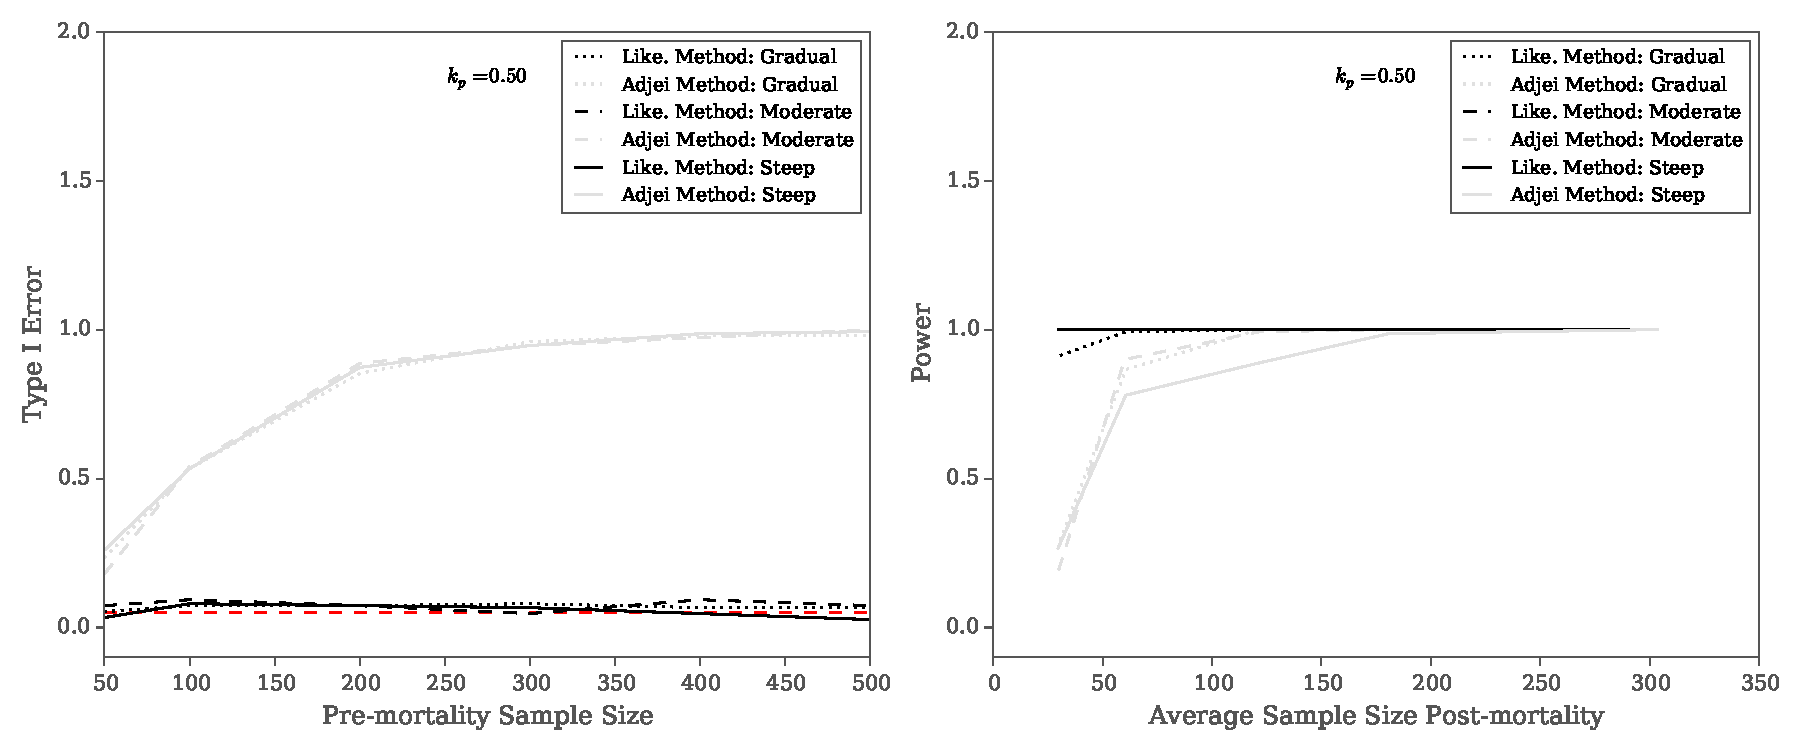
\includegraphics{/Users/mqwilber/Repos/parasite_mortality/results/figure1_partII_for_manuscript50}};

    \node[above=1cm] at (pic.north) (concept) {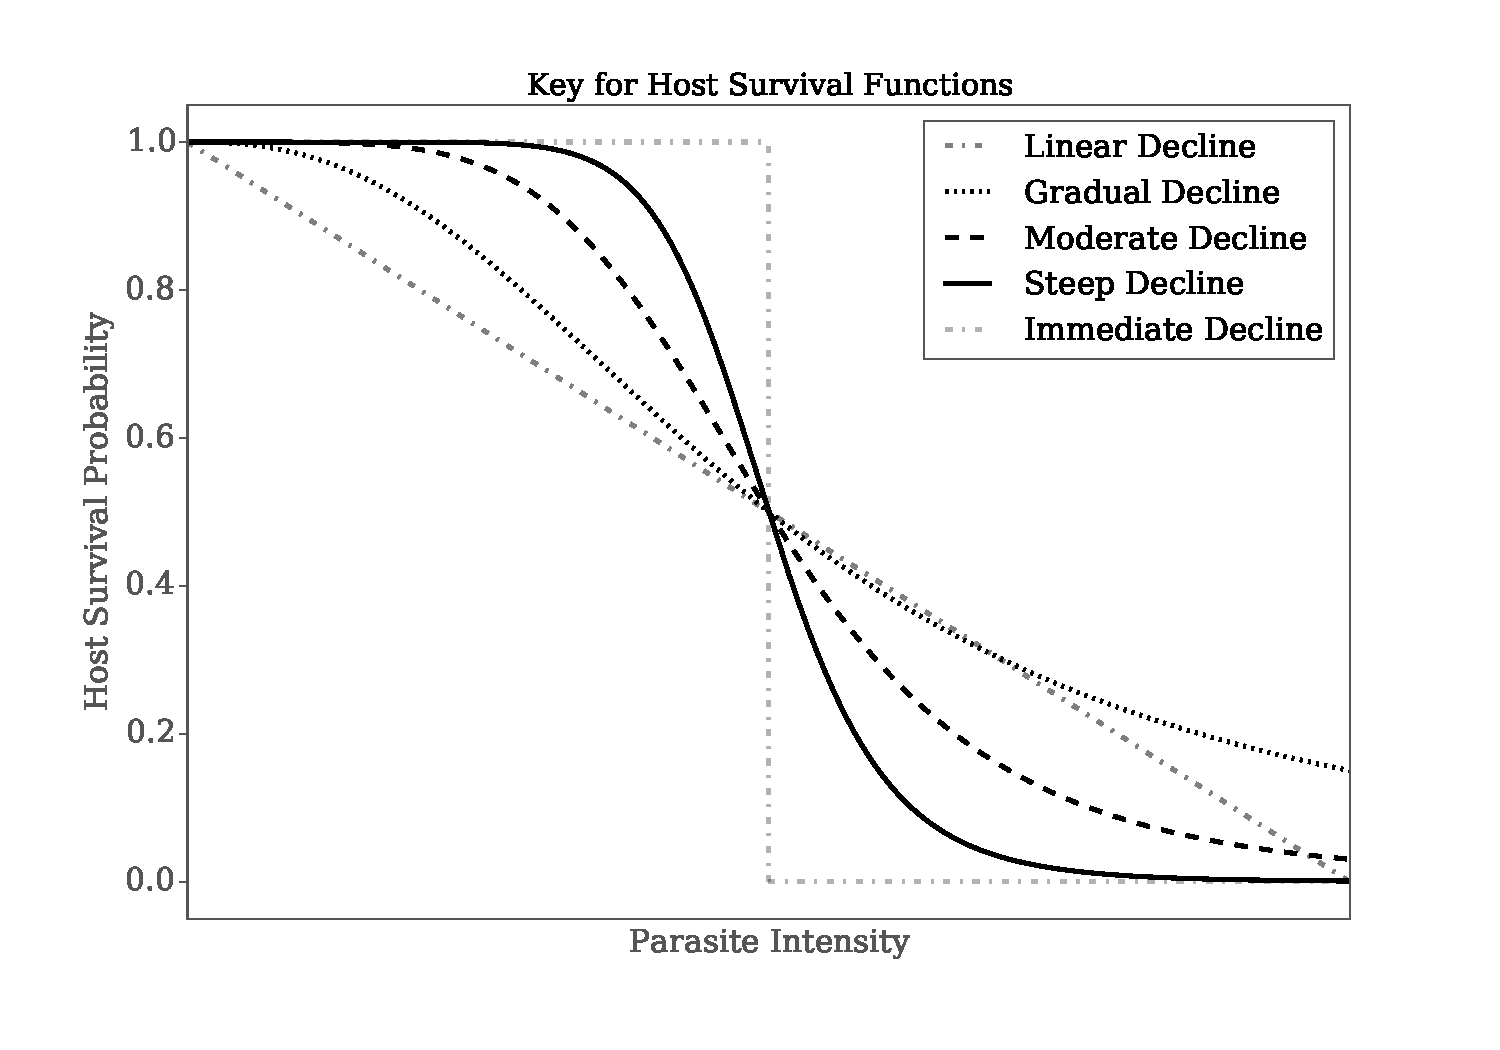
\includegraphics{/Users/mqwilber/Repos/parasite_mortality/results/figure1_partI_for_manuscript}};

    \node[above=1.3cm, at=(concept.south)] (temp) {};
    \node[right=6cm, at=(pic.north)] (right) {};
    \node[left=6cm, at=(pic.north)] (left) {};
    \draw[->, ultra thick]  (temp)--(right);
    \draw[->, ultra thick] (temp)--(left);

    \node at (-2.5, 3.8) {A};
    \node at (-5.1, 2.2) {B};
    \node at (0.9, 2.2) {C};

\end{tikzpicture}

\end{document}